BE and CF are two equal altitudes of a triangle ABC.
\captionsetup{justification=centering}
\begin{figure}[!h]
\centering
\resizebox{\columnwidth}{!}{


\tikzset{every picture/.style={line width=0.75pt}} %set default line width to 0.75pt        

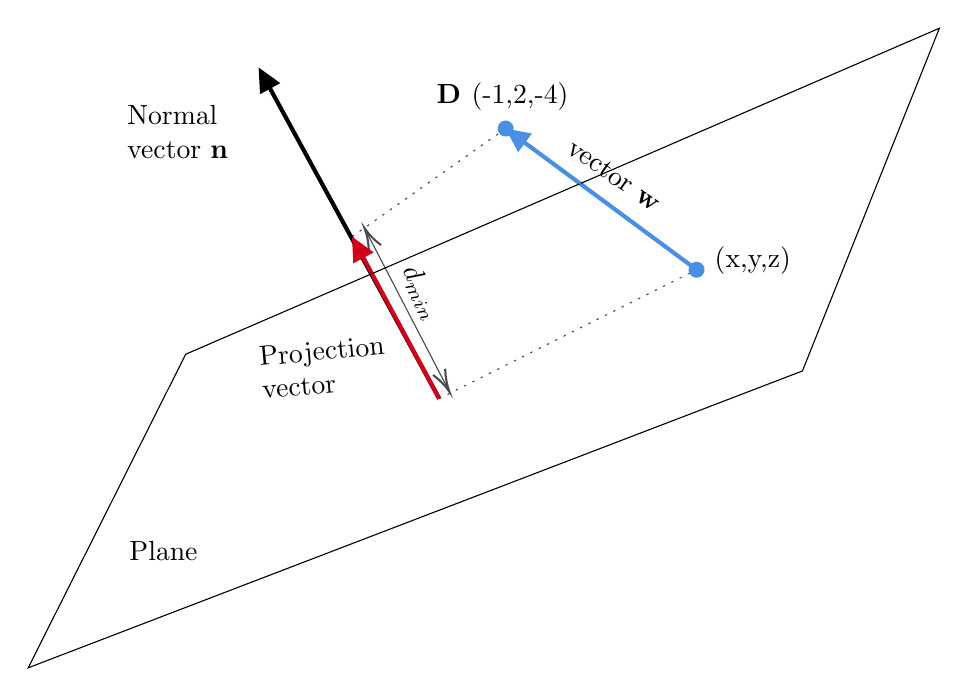
\begin{tikzpicture}[x=0.75pt,y=0.75pt,yscale=-1,xscale=1]
%uncomment if require: \path (0,324); %set diagram left start at 0, and has height of 324

%Straight Lines [id:da012474511036709712] 
\draw [color={rgb, 255:red, 74; green, 74; blue, 74 }  ,draw opacity=1 ] [dash pattern={on 0.84pt off 2.51pt}]  (165.51,108.36) -- (239.51,56.27) ;
%Straight Lines [id:da164610693713777] 
\draw [color={rgb, 255:red, 74; green, 74; blue, 74 }  ,draw opacity=1 ] [dash pattern={on 0.84pt off 2.51pt}]  (207.51,186.36) -- (331.51,124.27) ;
%Straight Lines [id:da0009900971082483778] 
\draw [color={rgb, 255:red, 74; green, 74; blue, 74 }  ,draw opacity=1 ]   (211.58,181.43) -- (172.42,105.98) ;
\draw [shift={(171.5,104.2)}, rotate = 422.57] [color={rgb, 255:red, 74; green, 74; blue, 74 }  ,draw opacity=1 ][line width=0.75]    (10.93,-3.29) .. controls (6.95,-1.4) and (3.31,-0.3) .. (0,0) .. controls (3.31,0.3) and (6.95,1.4) .. (10.93,3.29)   ;
\draw [shift={(212.5,183.2)}, rotate = 242.57] [color={rgb, 255:red, 74; green, 74; blue, 74 }  ,draw opacity=1 ][line width=0.75]    (10.93,-3.29) .. controls (6.95,-1.4) and (3.31,-0.3) .. (0,0) .. controls (3.31,0.3) and (6.95,1.4) .. (10.93,3.29)   ;
%Straight Lines [id:da6317108471264852] 
\draw [line width=1.5]    (207.51,186.36) -- (122.42,30.38) ;
\draw [shift={(120.51,26.87)}, rotate = 421.39] [fill={rgb, 255:red, 0; green, 0; blue, 0 }  ][line width=0.08]  [draw opacity=0] (11.61,-5.58) -- (0,0) -- (11.61,5.58) -- cycle    ;
%Straight Lines [id:da4711513779445873] 
\draw [color={rgb, 255:red, 74; green, 144; blue, 226 }  ,draw opacity=1 ][line width=1.5]    (331.51,124.27) -- (242.72,58.64) ;
\draw [shift={(239.51,56.27)}, rotate = 396.47] [fill={rgb, 255:red, 74; green, 144; blue, 226 }  ,fill opacity=1 ][line width=0.08]  [draw opacity=0] (11.61,-5.58) -- (0,0) -- (11.61,5.58) -- cycle    ;
%Straight Lines [id:da281513313013386] 
\draw [color={rgb, 255:red, 208; green, 2; blue, 27 }  ,draw opacity=1 ][line width=1.5]    (207.51,186.36) -- (167.4,111.89) ;
\draw [shift={(165.51,108.36)}, rotate = 421.7] [fill={rgb, 255:red, 208; green, 2; blue, 27 }  ,fill opacity=1 ][line width=0.08]  [draw opacity=0] (11.61,-5.58) -- (0,0) -- (11.61,5.58) -- cycle    ;
%Shape: Polygon [id:ds23253650680866844] 
\draw   (85.38,164.99) -- (448.5,7.93) -- (382.5,173.07) -- (9.5,316.07) -- (9.5,316.07) -- cycle ;
%Straight Lines [id:da02842289374539675] 
\draw [color={rgb, 255:red, 74; green, 144; blue, 226 }  ,draw opacity=1 ]   (239.51,56.27) -- (331.51,124.27) ;
\draw [shift={(331.51,124.27)}, rotate = 36.47] [color={rgb, 255:red, 74; green, 144; blue, 226 }  ,draw opacity=1 ][fill={rgb, 255:red, 74; green, 144; blue, 226 }  ,fill opacity=1 ][line width=0.75]      (0, 0) circle [x radius= 3.35, y radius= 3.35]   ;
\draw [shift={(239.51,56.27)}, rotate = 36.47] [color={rgb, 255:red, 74; green, 144; blue, 226 }  ,draw opacity=1 ][fill={rgb, 255:red, 74; green, 144; blue, 226 }  ,fill opacity=1 ][line width=0.75]      (0, 0) circle [x radius= 3.35, y radius= 3.35]   ;

% Text Node
\draw (56,44) node [anchor=north west][inner sep=0.75pt]   [align=left] {Normal \\vector \textbf{n} };
% Text Node
\draw (118.97,160.37) node [anchor=north west][inner sep=0.75pt]  [rotate=-354.79] [align=left] {Projection \\vector};
% Text Node
\draw (205,33) node [anchor=north west][inner sep=0.75pt]   [align=left] {\textbf{D }(-1,2,-4)};
% Text Node
\draw (339,112) node [anchor=north west][inner sep=0.75pt]   [align=left] {(x,y,z)};
% Text Node
\draw (272.66,59.12) node [anchor=north west][inner sep=0.75pt]  [rotate=-34.52] [align=left] {vector \textbf{w} };
% Text Node
\draw (198.69,119.24) node [anchor=north west][inner sep=0.75pt]  [rotate=-64.65] [align=left] {$d_{min}$};
% Text Node
\draw (57,254.07) node [anchor=north west][inner sep=0.75pt]   [align=left] {Plane};


\end{tikzpicture}
}
\caption{Triangle with equal altitudes on two sides}
\label{eq:solutions/1/36/myfig}
\end{figure}
Given:-\\
1) Altitudes are Equal means their magnitude are same
 \begin{align}
 	\norm{\vec{E} - \vec{B}} = \norm{\vec{F} - \vec{C}} \label{eq:solutions/1/36/1}
 \end{align}
2) Altitude makes right angle at the base therefore $\cos 90 =0$ therefore  FC $\perp$ BF and EB $\perp$ CE where $\textbf{m}$ is the directional vectors.
\begin{align}
\textbf{m}_{FC} \textbf{m}_{BF} = 0 \label{eq:solutions/1/36/2}\\
\textbf{m}_{EB} \textbf{m}_{CE} = 0 \label{eq:solutions/1/36/3}
\end{align}
From \eqref{eq:solutions/1/36/2}
\begin{align}
    \brak{\vec{B}-\vec{F}}^T\brak{\vec{F}-\vec{C}}=\vec{0} && \brak{\vec{F}-\vec{C}}^T\brak{\vec{B}-\vec{F}}=\vec{0}\label{eq:solutions/1/36/4}
\end{align}
From \eqref{eq:solutions/1/36/2} and using \eqref{eq:solutions/1/36/4} 
\begin{align}
    \brak{\vec{B}-\vec{C}}^T\brak{\vec{B}-\vec{C}}\\
    =\brak{\vec{B}-\vec{F}+\vec{F}-\vec{C}}^T\brak{\vec{B}-\vec{F}+\vec{F}-\vec{C}})
    \end{align}
    \begin{align}
      =\brak{\vec{B}-\vec{F}}^T\brak{\vec{B}-\vec{F}}+\brak{\vec{F}-\vec{C}}^T\brak{\vec{F}-\vec{C}} 
    \end{align}
\begin{align}
   \norm{\vec{B}-\vec{C}}^2=\norm{\vec{B}-\vec{F}}^2+\norm{\vec{F}-\vec{C}}^2\label{eq:solutions/1/36/8} 
    \end{align}
    Similarly\\
    From \eqref{eq:solutions/1/36/3}
    \begin{align}
        \brak{\vec{E}-\vec{B}}^T\brak{\vec{E}-\vec{C}}=\vec{0} && \brak{\vec{E}-\vec{C}}^T\brak{\vec{B}-\vec{E}}=\vec{0}\label{eq:solutions/1/36/9}
        \end{align}
From  \eqref{eq:solutions/1/36/3} and using \eqref{eq:solutions/1/36/9}  
\begin{align}
    \brak{\vec{B}-\vec{C}}^T\brak{\vec{B}-\vec{C}}\\
    =\brak{\vec{B}-\vec{E}+\vec{E}-\vec{C}}^T\brak{\vec{B}-\vec{E}+\vec{E}-\vec{C}}
    \end{align}
    \begin{align}
      =\brak{\vec{B}-\vec{E}}^T\brak{\vec{B}-\vec{E}}+\brak{\vec{E}-\vec{C}}^T\brak{\vec{E}-\vec{C}} 
    \end{align}
\begin{align}
   \norm{\vec{B}-\vec{C}}^2=\norm{\vec{B}-\vec{E}}^2+\norm{\vec{E}-\vec{C}}^2\label{eq:solutions/1/36/13}
    \end{align}        
    Equating \eqref{eq:solutions/1/36/8} and \eqref{eq:solutions/1/36/13} and using \eqref{eq:solutions/1/36/1}
    \begin{align}
      \norm{\vec{B}-\vec{F}}^2+\norm{\vec{F}-\vec{C}}^2 = \norm{\vec{B}-\vec{E}}^2+\norm{\vec{E}-\vec{C}}^2  
    \end{align}
    \begin{align}
       \norm{\vec{B}-\vec{F}}^2=\norm{\vec{E}-\vec{C}}^2\\
       =\norm{\vec{B}-\vec{F}}=\norm{\vec{E}-\vec{C}}\label{eq:solutions/1/36/16}
    \end{align}
Let $\angle FBC=\theta_1$  and  $\angle EBC=\theta_2$
    \begin{align}
        \brak{\vec{B}-\vec{F}}^T\brak{\vec{B}-\vec{C}}=\norm{\vec{B}-\vec{F}}\norm{\vec{B}-\vec{C}}\cos\theta_1\\
        \cos{\theta_1}=\frac{\brak{\vec{B}-\vec{F}}^T\brak{\vec{B}-\vec{C}}}{\norm{\vec{B}-\vec{F}}\norm{\vec{B}-\vec{C}}}\\
        \cos{\theta_1}=\frac{\brak{\vec{B}-\vec{F}}^T\brak{\vec{B}-\vec{F}+\vec{F}-\vec{C}}}{\norm{\vec{B}-\vec{F}}\norm{\vec{B}-\vec{C}}}\\
        \cos{\theta_1}=\frac{\brak{\vec{B}-\vec{F}}^T\brak{\vec{B}-\vec{F}} +\brak{\vec{B}-\vec{F}}^T\brak{\vec{F}-\vec{C}}}{\norm{\vec{B}-\vec{F}}\norm{\vec{B}-\vec{C}}}
        \end{align}
        From \eqref{eq:solutions/1/36/4}
        \begin{align}
          \cos{\theta_1}=\frac{\brak{\vec{B}-\vec{F}}^T\brak{\vec{B}-\vec{F}}}{\norm{\vec{B}-\vec{F}}\norm{\vec{B}-\vec{C}}} \\
          \cos{\theta_1}=\frac{\norm{\vec{B}-\vec{F}}^2}{\norm{\vec{B}-\vec{F}}\norm{\vec{B}-\vec{C}}}\\
          \cos{\theta_1}=\frac{\norm{\vec{B}-\vec{F}}}{\norm{\vec{B}-\vec{C}}}
        \end{align}
        Similarly for $\angle EBC=\theta_2$
       \begin{align}
        \brak{\vec{C}-\vec{E}}^T\brak{\vec{B}-\vec{C}}=\norm{\vec{C}-\vec{E}}\norm{\vec{B}-\vec{C}}\cos\theta_2\\
        \cos{\theta_2}=\frac{\brak{\vec{C}-\vec{E}}^T\brak{\vec{B}-\vec{C}}}{\norm{\vec{C}-\vec{E}}\norm{\vec{B}-\vec{C}}}\\
        \cos{\theta_2}=\frac{\brak{\vec{C}-\vec{E}}^T\brak{\vec{B}-\vec{E}+\vec{E}-\vec{C}}}{\norm{\vec{C}-\vec{E}}\norm{\vec{B}-\vec{C}}}\\
        \cos{\theta_2}=\frac{\brak{\vec{C}-\vec{E}}^T\brak{\vec{B}-\vec{E}} +\brak{\vec{C}-\vec{E}}^T\brak{\vec{E}-\vec{C}}}{\norm{\vec{C}-\vec{E}}\norm{\vec{B}-\vec{C}}}
        \end{align}
        From {\eqref{eq:solutions/1/36/9}}
        \begin{align}
          \cos{\theta_2}=\frac{\brak{\vec{C}-\vec{E}}^T\brak{\vec{C}-\vec{E}}}{\norm{\vec{C}-\vec{E}}\norm{\vec{B}-\vec{C}}} \\
          \cos{\theta_2}=\frac{\norm{\vec{C}-\vec{E}}^2}{\norm{\vec{C}-\vec{E}}\norm{\vec{B}-\vec{C}}}\\
          \cos{\theta_2}=\frac{\norm{\vec{C}-\vec{E}}}{\norm{\vec{B}-\vec{C}}}
        \end{align}
        From \eqref{eq:solutions/1/36/16} we know $\norm{\vec{B}-\vec{F}}=\norm{\vec{E}-\vec{C}}$ we conclude
        \begin{align}
            \cos\theta_1=\cos\theta_2
            \implies\theta_1=\theta_2
        \end{align}
        So the sides opposite to equal angles are equal. Hence AB=AC hence the given Triangle is isosceles.
